%%%%%%%%%%%%%%%%%%%%%%%%%%%%%%%%%%%%%%%%%%%%%%%%%%%%%%%%%%%%%%%%%%%%%%%%%%%%%%%%
\chapter{Related Work}
\label{chapter:p1-ch3-related_work}
%%%%%%%%%%%%%%%%%%%%%%%%%%%%%%%%%%%%%%%%%%%%%%%%%%%%%%%%%%%%%%%%%%%%%%%%%%%%%%%%
\localtableofcontents

%%%%%%%%%%%%%%%%%%%%%%%%%%%%%%%%%%%%%%%%%%%%%%%%%%%%%%%%%%%%%%%%%%%%%%%%%%%%%%%%
\section{Introduction}
\label{section:p1-ch3_introduction}
%%%%%%%%%%%%%%%%%%%%%%%%%%%%%%%%%%%%%%%%%%%%%%%%%%%%%%%%%%%%%%%%%%%%%%%%%%%%%%%%


% comment on compte le numbre de parametre d'un réseau 
% ce qui nous interesse, ce n'est pas le nombre de parametre mais le nombre de parametre necessaire de stocker en mémoire 
% deux techniques: soit on prune le network a posteriori et dans ce cas, on utilise des reprséenytation informatique matricielle sparse
% ou alors on utilise des matrices structurées qui sont utilise des opérations d'algèbre lineraire spécifiqie 

% One method consist of building compact architecture: reducing the input and hidden layers dimension and reducing the depth of the network.
% reduce the dimension of the hidden layer and/or reduce the depth of the network. 

In this chapter, we review the literature on the existing techniques for building compact neural networks.
As stated in the introduction (Chapter~\ref{chapter:ch1-introduction}), a neural network is a function that can be analytically described as a composition of linear functions interlaced with non-linear functions (also called activation functions).
% Therefore, a neural network $f_\Theta : \Rbb^n \rightarrow \Rbb^m$ can be defined as follows:
% \begin{equation}
%   f_\Theta(\xvec) \triangleq \phi_{\Wmat^{(p)}} \circ \rho \circ \phi_{\Wmat^{(p-1)}} \circ \cdots \circ \phi_{\Wmat^{(2)}} \circ \rho \circ \phi_{\Wmat^{(1)}}(\xvec)
%   \label{equation:p1-ch3_neural_network}
% \end{equation}
% where $p$ corresponds to the \emph{depth} of the network (\ie, the number of layers), the function $\phi_{\Wmat^{(i)}}$ is a linear function parameterized by $\Wmat^{(i)}$, $\rho$ is a non-linear function and $\Theta \triangleq \left( \Wmat^{(1)}, \dots, \Wmat^{(p)} \right)$.
% The input space $n$ corresponds to the dimension of the data and the output space $m$ corresponds to the number of classes the network has to classify.
Therefore, a neural network $f_{\Theta,\Bmat} : \Rbb^n \rightarrow \Rbb^m$ can be defined as follows:
\begin{equation}
  f_{\Theta,\Bmat}(\xvec) \triangleq \phi_{\Wmat^{(L)}, \bvec^{(L)}} \circ \cdots \circ \phi_{\Wmat^{(1)}, \bvec^{(1)}}(\xvec)
  \label{equation:p1-ch3_neural_network}
\end{equation}
where $L$ corresponds to the \emph{depth} of the network (\ie, the number of layers), $\Theta$ is the set of weights matrices $\Theta \triangleq \left( \Wmat^{(1)}, \dots, \Wmat^{(L)} \right)$, $\Bmat$ is the set of bias vectors $\Bmat \triangleq \left( \bvec^{(1)}, \dots, \bvec^{(L)} \right)$ and the function $\phi_{\Wmat^{(i)},\bvec^{(i)}}$ is define by: $\phi_{\Wmat^{(i)},\bvec^{(i)}} \triangleq \rho\left(\Wmat^{(i)}\xvec + \bvec^{(i)}\right)$ where $\rho$ is a non-linear function.


The number of parameters in a neural network corresponds to the total number of values in each weight matrix of the network.
The goal of building compact neural networks is to reduce the memory footprint, the number of parameters and the computational complexity of the network. 
Mainly three methods exist to achieve this goal:
\begin{itemize}
  \item Leveraging memory representations and data structures;
  \item Using structured matrices instead of dense matrices;
  \item Building compact neural networks architecture.
\end{itemize}
Hereafter, we describe existing techniques that fall into these categories and we review their advantages and their drawbacks.


%%%%%%%%%%%%%%%%%%%%%%%%%%%%%%%%%%%%%%%%%%%%%%%%%%%%%%%%%%%%%%%%%%%%%%%%%%%%%%%%
\section{Leveraging Memory Representations and Data Structures}
\label{section:p1-ch3-leveraging_memory_representations_and_data_structures}
%%%%%%%%%%%%%%%%%%%%%%%%%%%%%%%%%%%%%%%%%%%%%%%%%%%%%%%%%%%%%%%%%%%%%%%%%%%%%%%%

% leverging programming techniques
% prunning => need to levrage the spasity of matrices in order to reduce memory 
% sparsity regularizers => same

An effective method to make a compact neural network is to use programming tools and techniques to reduce their memory representation. 
Indeed, when we use a neural network in a computer system, we need to define the memory representation of the weights and the data structure to use.
One of the most widely used memory representations for numerical values is the single-precision floating-point format which uses 32 bits of computer memory.
Researchers have noticed that a high precision of neural networks weights might not be necessary and have tried to use different representations.
\citet{gupta2015deep} were one of the first to train neural networks with limited numerical precision in order to save memory.
They use half-precision floating-point format which used 16 bits instead of 32.
This work offers a trade-off between the expressivity of the neural network governed by the weights precision and the accuracy.
More recently, \citet{micikevicius2018mixed} have built on the work of~\citet{gupta2015deep} and proposed training neural networks with mixed precision floating format.
They proposed to use both single and half precision in order to have a more fine-grained control over the trade-off compression/accuracy.

Using half-precision floating-point format is not the only format available to computer scientists to reduce memory.
Binary and integer formats can take even fewer bits in computer memory.
Recently, \citet{courbariaux2015binaryconnect} have proposed a method to train neural networks with binary weights.
While this approach can significantly reduce the memory footprint of neural networks, it is difficult to maintain the binary constraint during training. 
Moreover, an important idea in model compression, proposed by~\citet{bucilua2006model}, is based on the observation that the model used for training is not required to be the same as the one used for inference, indeed, compressed models after training can be deployed on smartphones or IoT devices.
Based on this idea, researchers \cite{mellempudi2017ternary,rastegariECCV16} have proposed a quantization procedure which consists of converting the weights into a binary or integer formats \emph{after} the training phase. 


% Using half-precision floating-point format is not the only format available to computer scientists to reduce memory.  
% Binary and integer formats can take even fewer bits in computer memory.
% However, it is difficult to constraints the training of neural networks with weights being either integers or binary.
%
% Even though using binary and integer formats could considerably reduce the memory footprint of neural networks, it is difficult to maintain this constrain during training.
% Indeed, the training of neural network is based on stochastic gradient descent 
%
% constraints the training of neural networks with weights being either integers or binary. 
%
% Moreover, an important idea in model compression, proposed by~\citet{bucilua2006model}, is based on the observation that the model used for training is not required to be the same as the one used for inference.
% Following these constraints and ideas, researchers have come up with several ways of compressing neural networks after training. 
% One of these techniques~\cite{courbariaux2015binaryconnect,mellempudi2017ternary,rastegariECCV16} consists of using binary or integer formats after a quantization procedure of the neural network weights after training. 
%
%
% This still requires that the large model be trained with the current drawbacks (difficulty and cost of training) but compressed models after training can be deployed on smartphones or IoT devices.





\begin{table}[t]
  \centering
  {\small
  \begin{tabular}{llcc}
    \toprule
    \textbf{Authors} & \textbf{Models} & \textbf{Baseline} & \textbf{Mixed Precision} \\
    \midrule
    \citet{krizhevsky2012imagenet} & AlexNet & 56.77\% & 56.93\% \\
    \citet{simonyan2014very} & VGG & 65.40\% & 65.43\% \\
    \citet{szegedy2015going} & GoogLeNet & 68.33\% & 68.43\% \\
    \citet{ioffe2015batch} & Inception v2 & 70.03\% & 70.02\% \\
    \citet{szegedy2016rethinking} & Inception v3 & 73.85\% & 74.13\% \\
    \citet{he2016deep} & Resnet50 & 75.92\% & 76.04\% \\
    \bottomrule
  \end{tabular}
  }
  \caption{Comparison of TOP-1 Accuracy on the ImageNet Dataset \cite{deng2009imagenet} between baseline training and mixed precision training \cite{micikevicius2018mixed}.}
  \label{table:p1-ch3-basline_vs_mixed_precision}
\end{table}


Another widely used technique to compress neural network after the training phase is to use sparse data structures for weights matrices.
Indeed, it has been observed that redundant parameters can be omitted from the model without significantly changing the accuracy.
These observations have led to pruning techniques~\cite{dai2018compressing,han2015deep,lin2017runtime} or sparsity regularizers~\cite{collins2014memory,dai2018compressing,liu2015sparse} which consists of removing useless weights after training and leveraging the sparse structure of the weights matrices.
Sparse neural networks have been extensively studied since the \emph{Lottery Ticket Hypothesis} proposed by \citet{frankle2018lottery}.
This hypothesis states that it exists a sparse neural network \ie, a subnetwork of dense neural network, that when trained in isolation can match the test accuracy of the original dense network after training for at most the same number of iterations.
This hypothesis led to a series of works on sparse neural networks \cite{zhou2019deconstructing,malach2019proving,evci2020rigging}.

Other original techniques have been designed to reduce the number of parameters used in neural networks. 
\citet{chen2015compressing} have proposed to compress weight matrices by using hash functions to map several matrix coefficients into the same memory cell.
However, in practice, hashing techniques are difficult to use because of their irregular memory access patterns which makes them inadequate for GPU execution.



% % prunning
% To compress an existing network several researchers have investigated techniques to prune parameters that are redundant (\eg ~\cite{dai2018compressing,han2015deep,lin2017runtime}).
%
% It is also possible to use sparsity regularizers during training, to be able to compress the model after the training using efficient sparse matrix representations (\eg~\cite{collins2014memory,dai2018compressing,liu2015sparse}).

% One of this techniques consists of using binary or integer formats following a quantization step of the neural network weights after training. 
%
% works~\cite{courbariaux2015binaryconnect,mellempudi2017ternary,rastegariECCV16} have proposed to use binary or integer formats with a quantization step of the neural network weights after training.
%

% quantization~\cite{courbariaux2015binaryconnect,mellempudi2017ternary,rastegariECCV16} techniques that consists of converting the weights single-precision format to a integer or binary format after training.
%
% Researchers have noticed that the model used for training is not required to be the same as the one used for inference.

% Howevee, given that it is difficult to constraint the training  
%
% quantization \cite{courbariaux2015binaryconnect,mellempudi2017ternary,rastegariECCV16}



%%%%%%%%%%%%%%%%%%%%%%%%%%%%%%%%%%%%%%%%%%%%%%%%%%%%%%%%%%%%%%%%%%%%%%%%%%%%%%%%
\section{Compact Neural Networks with Structured Matrices}
\label{section:p1-ch3-compact_neural_networks_with_structured_matrices}
%%%%%%%%%%%%%%%%%%%%%%%%%%%%%%%%%%%%%%%%%%%%%%%%%%%%%%%%%%%%%%%%%%%%%%%%%%%%%%%%


Another way of constraining the weight representation and reduce the memory requirement of neural networks is to impose a \emph{structure} on weight matrices. 
% The layers of a neural network are a simple linear transform combined with a non-linear function (\eg, ReLU function). 
% The neural network $f_\Theta$ presented in Equation~\ref{equation:p1-ch3_neural_network} can be described with the recurrent relation as follows:
% \begin{align}
%   \xvec^{(1)} &= \xvec \\
%   \xvec^{(i+1)} &= \rho\left( \Wmat^{(i)} \xvec^{(i)} \right) \\
%   f_\Theta(\xvec) &= \xvec^{(p)}
% \end{align}
% $\xvec^{(i)}$ is the $i$ layer of the neural network $f_\Theta$.
The idea of building compact neural networks with structured matrices consists of replacing the weight matrices $\Wmat^{(i)}$ with \emph{structured matrices}.

A structured matrix is a $n \times n$ matrix whose entries have a formulaic relationship, allowing the matrix to be represented with fewer than $n^2$ parameters.
The formulaic relationship between entries is an important feature to consider, for example, a sparse matrix has fewer than $n^2$ parameters but does not have a clear relationship between its entries.

A classic example of structured matrices are \emph{low-rank} matrices which result from the product of two rectangular matrices.
Let $\Umat, \Vmat \in \Rbb^{n \times m}$ with $n < m$, the matrix $\Wmat = \Umat^\top \Vmat$ will be low-rank with rank $n$.
\citet{denil2013predicting} were among the first to use low-rank matrices in deep learning contexts followed by the work of~\citet{jaderberg2014speeding,yu2017compressing}.
They replaced the dense weight matrices $\Wmat^{(i)}$ with a product of two rectangular matrices $\Umat^{(i)}, \Vmat^{(i)} \in \Rbb^{n \times m}$ with $n < m$ which led to neural network layer defined as follows:
\begin{equation}
  \xvec^{(i+1)} = \rho\left( \Umat^{(i)\top} \Vmat^{(i)} \xvec^{(i)} \right) .
\end{equation}
By replacing the dense weight matrices $\Wmat^{(i)}$ with the product of two rectangular matrices and learning them instead of the dense matrices, they \emph{impose} on the learning procedure the low-rank constraint.
We can remark that the matrix resulting from the product of $\Umat^{(i)\top} \Vmat^{(i)}$ has $n^2$ unique values but can still be represented with only $2nm$ values in memory.

in linear algebra, many structures have been discovered and studied~\cite{pan2001structured}. 
for example, circulant matrices have been used to efficiently solve linear systems~\cite{golub1996matrix} and years later were used to perform dimensionality reduction~\cite{hinrichs2011johnson,vybiral2011variant}, binary embedding~\cite{yu2014circulant} and kernel approximation~\cite{yu2015compact} in the context of pattern recognition and machine learning.
an $n \times n$ circulant matrix $\cmat$ is a matrix where each row is a cyclic right shift of the previous one:
\begin{equation}
  \cmat = \leftmatrix
  \cvec_{0} & \cvec_{n-1} & \dots & \cvec_{1} \\
  \cvec_{1} & \cvec_{0} & \dots & \cvec_{2} \\
  \vdots & \vdots & \ddots & \vdots \\
  \cvec_{n-1} & \cvec_{n-2} & \dots & \phantom{0}\cvec_{0}\phantom{0}
  \rightmatrix
\end{equation}
because the circulant matrix $\cmat$ is fully determined by the vector $\cvec$, it can be compactly represented in memory using only $n$ values instead of $n^2$.
circulant matrices can also be characterized by noting that the $(k,j)$ entry of $\cmat$, $\cmat_{j,k}$ is given by
\begin{equation}
  \cmat_{j,k} = \cvec_{\left(k-j\right) \mod n} \enspace.
\end{equation}
circulant matrices exhibit several interesting properties which are based on the fact that they can be diagonalized by the discrete fourier transform (dft)~\cite{davis1979circulant}.
more precisely, the eigenvalues $\psi_k$ of the matrix $\cmat$ correspond to the discrete fourier transform of the vector characteristic $\cvec$:
\begin{equation}
  \mathbf{\psi}_k = \sum_{j=0}^{n-1} c_j e^{-\frac{2 \pi \ci}{n} jk}
\end{equation}
and the eigenvectors $\yvec^{(k)}$ can be expressed as follows:
\begin{equation}
  \yvec^{(k)} = \frac{1}{\sqrt{n}} \leftmatrix 1, e^{-\frac{2 \pi \ci k}{n}}, \dots, e^{-\frac{2 \pi \ci k(n-1)}{n}} \rightmatrix^\top
\end{equation}
in matrix form, we can diagonalize the matrix $\cmat$ as follows:
\begin{equation}
  \cmat = \frac{1}{n} \umat_n^{-1} \diag(\umat_n \cvec) \umat_n
\end{equation}
where $\umat_n = \leftmatrix e^{-\frac{2 \pi \ci jk}{n}} \rightmatrix_{j,k = 0}^{n-1}$ is the dft matrix.
the complexity of the matrix-vector product between a circulant matrix $\cmat$ and a vector $\xvec$ can be reduced from $o(n^2)$ to $o(n \log n)$ with the \emph{fast fourier transform} algorithm~\cite{cooley1965algorithm}.


% An additional benefit of circulant matrices, is that they are computationally efficient, especially on GPU devices.
% Multiplying a circulant matrix $C$ by a vector $x$ is equivalent to a circular convolution between $c$ and $x$ (denoted $c \star x$).
% Furthermore, the circular convolution can be computed in the Fourier domain as follows. 

% Most importantly, any $n \times n$ circulant matrix $\Cmat$ can be represented using only $n$ coefficients instead of the $n^2$ coefficients required to represent classical unstructured matrices.

% For example, \citet{hinrichs2011johnson} have demonstrated that a single circulant matrix can be used to approximate the Johnson-Lindenstrauss transform, often used in machine learning to perform dimensionality reduction.

% From these properties and previous applications, \citet{cheng2015exploration} had the idea to replace the weight matrix of a fully connected layer by a circulant matrix 


From these properties and previous applications, \citet{cheng2015exploration} had the idea to replace the weight matrix of a fully connected layer by circulant and diagonal matrices where the circulant matrix is learned by a gradient-based optimization algorithm and the diagonal matrix entries are sampled at random in $\{-1, 1\}$.
This effectively replaces the complex transform modeled by the fully connected layer by a simple dimensionality reduction.
Despite the reduction of expressivity, their experiments demonstrated good accuracy using only a fraction of the original size of the network (90\% reduction).
Indeed, the last 3 fully connected layers of the AlexNet~\cite{krizhevsky2012imagenet} architecture use 58M out of the 62M total trainable parameters ($> 90\%$ of the total number of parameters).

\citet{moczulski2016acdc} build upon the work of~\citet{cheng2015exploration} and introduced two \emph{Structured Efficient Linear Layers} (SELL) called \AFDF and \ACDC, where $\Amat$ and $\Dmat$ are diagonal matrices and $\Fmat$ and $\Cmat$ are the Fourier and cosine transform respectively.
Their work is two-fold, first, they theoretically study the \AFDF linear layer which consists of a diagonal matrix \eg, the matrix $\Dmat$ and a circulant matrix \eg, the decomposition $\mathbf{FDF}^{-1}$.
Then they experiment using the \ACDC linear layer which consists of a diagonal matrices \eg, the matrices $\Amat$ and $\Dmat$ interlaced with the cosine transform.
As far as we can tell, the theoretical guarantees available for the \AFDF layer do not apply to the \ACDC layer since the cosine transform does not diagonalize circulant matrices \cite{sanchez1995diagonalizing}.
Although the resulting network demonstrates good accuracy, it is difficult to characterize the true contribution of the \ACDC layers in this setting. 

\begin{figure}[t]
   \centering
   \begin{subfigure}[b]{0.32\textwidth}
       \centering
       \begin{equation*}
	  \leftmatrix
	    t_0 & t_{1} & \cdots & t_{n-1}  \\
	    t_{-1} & t_0 & \ddots & \vdots \\
	    \vdots & \ddots & \ddots & t_{1} \\
	    t_{-n+1} & \cdots & t_{-1} & t_0
	  \rightmatrix
       \end{equation*}
       \caption*{Toeplitz}
   \end{subfigure}
   \hfill
   \begin{subfigure}[b]{0.32\textwidth}
       \centering
       \begin{equation*}
	  \leftmatrix
	    1 & v_0 & \cdots & v_0^{n-1} \\
	    1 & v_1 & \cdots & v_1^{n-1} \\
	    1 & \vdots & & \vdots \\
	    1 & v_{n-1} & \cdots & v_{n-1}^{n-1}
	  \rightmatrix
       \end{equation*}
       \caption*{Vandermonde}
   \end{subfigure}
   \hfill
   \begin{subfigure}[b]{0.32\textwidth}
       \centering
       \begin{equation*}
	  \leftmatrix
	  \frac{1}{u_0 - v_{0}} & \cdots & \frac{1}{u_0 - v_{n-1}} \\
	  \frac{1}{u_1 - v_{0}} & \cdots & \frac{1}{u_1 - v_{n-1}} \\
	  \vdots & \cdots & \vdots \\
	  \frac{1}{u_{n-1} - v_{0}} & \cdots & \frac{1}{u_{n-1} - v_{n-1}} \\
	  \rightmatrix
       \end{equation*}
       \caption*{Cauchy}
   \end{subfigure}
   \caption{Structured matrices that can be characterized by a low displacement rank.}
  \label{figure:p1-ch3_example_structure_matrices}
\end{figure}

Around the same time, \citet{sindhwani2015structured} used circulant matrices and other type of structured matrices \eg, Toeplitz, Vandermonde, and Cauchy matrices (see Figure~\ref{figure:p1-ch3_example_structure_matrices}) to train compact neural networks for keyword spotting applications in mobile speech recognition.
They proposed a unified framework of structured matrices that are characterized by the notion of low displacement rank.
Their methods demonstrate that compact neural networks with structured matrices are much more effective than standard linear low-rank bottleneck layers.

More recently, \citet{thomas2018learning} have generalized these works by training neural networks with low-displacement rank matrices (LDR), that are structured matrices encompassing a large family of structured matrices, including Toeplitz-like, Vandermonde-like, Cauchy-like.
To obtain this result, LDR represents a structured matrix using two displacement operators and a low-rank residual.
Despite being elegant and general, we found that the LDR framework suffers from several limits which are inherent to its generality and makes it difficult to use in the context of large and deep neural networks.
First, the training procedure for learning LDR matrices is highly involved and implies many complex mathematical objects such as Krylov matrices.
Then, as acknowledged by the authors, the number of parameters required to represent a given structured matrix (a Toeplitz matrix) in practice is unnecessarily high (higher than required in theory). 

Other, more complex, structured projections have been used in the context of compact neural networks.
The Fastfood transform~\cite{le2013fastfood}, which was originally used for approximating kernel expansions, was later used in neural networks by~\citet{yang2015deep} leading to the Deep Fried Convnets architecture.
The authors have replaced dense matrices of fully connected layers with adaptative structured matrices of the form: $\Smat\Hmat\Gmat\mathbf{\Pi}\Hmat\Bmat$ where $\Smat$, $\Gmat$, and $\Bmat$ are adaptive diagonal matrices, $\mathbf{\Pi}$ is a random permutation matrix, and $\Hmat$ is the Walsh-Hadamard matrix.
Later, the \emph{Structured Spinners} transform of the form: $\Hmat\Dmat_3\Hmat\Dmat_2\Hmat\Dmat_1$, where $\Hmat$ is the Walsh-Hadamard matrix, and $\Dmat_i$ for $i \in {1, 2, 3}$ is a random $\pm1$-diagonal matrix, was originally proposed by~\citet{andoni2015practical} and used in deep learning settings by~\citet{bojarski2017structured}.
In the same vein, \citet{novikov2015tensorizing} have proposed to replace the dense weight matrices of fully connected layers by the \emph{Tensor Train decomposition} allowing an important reduction of the number of parameters while preserving the expressive power of the layers.



% In this paper we convert the dense weight matrices of the fully connected layers to the Tensor Train format such that the number of parameters is reduced by a huge factor and at the same time the expressive power of the layer is preserved


% The \AFDF structured layer benefits from the theoretical results introduced by \citet{huhtanen2015factoring} and can be seen as the building block of DCNNs.
% However, \citet{moczulski2016acdc} only experiment using \ACDC, a different type of layer that does not involve circulant matrices.
% As far as we can tell, the theoretical guarantees available for the \AFDF layer do not apply on the \ACDC layer since the cosine transform does not diagonalize circulant matrices \cite{sanchez1995diagonalizing}.
% Another possible limit of the \ACDC paper is that they only train large neural networks involving \ACDC layers combined with many other expressive layers.

% using circulant matrices~\cite{cheng2015exploration,sindhwani2015structured}
% Vandermonde~\cite{sindhwani2015structured}


% More recently, \citet{thomas2018learning} have generalized these works by proposing neural networks with low-displacement rank matrices (LDR), that are structured matrices encompassing a large family of structured matrices, including Toeplitz-like, Vandermonde-like, Cauchy-like and more notably DCNNs.
% To obtain this result, LDR represents a structured matrix using two displacement operators and a low-rank residual.
% Despite being elegant and general, we found that the LDR framework suffers from several limits which are inherent to its generality and makes it difficult to use in the context of large and deep neural networks.
% First, the training procedure for learning LDR matrices is highly involved and implies many complex mathematical objects such as Krylov matrices.
% Then, as acknowledged by the authors, the number of parameters required to represent a given structured matrix (a Toeplitz matrix) in practice is unnecessarily high (higher than required in theory). 

% In this domain, \citet{cheng2015exploration} have proposed to replace two fully connected layers of AlexNet by circulant and diagonal matrices where the circulant matrix is learned by a gradient based optimization algorithm and the diagonal matrix entries are sampled at random in $\{-1, 1\}$. 

% The size of the model is reduced by a factor of 10 without loss in accuracy. 

% diagonalization of circulant matrix \cite{davis1979circulant}
%
% In addition, the matrix-vector product is simplified from $O(n^2)$ to $O(n \log n)$ using the convolution theorem.

% Because the circulant matrix $C \in \Rbb^{n\times n}$ is fully determined by the vector $c \in \Rbb^n$, the matrix $C$ can be compactly represented in memory using only $n$ real values instead of $n^2$.

% An additional benefit of circulant matrices, is that they are computationally efficient, especially on GPU devices.
% Multiplying a circulant matrix $C$ by a vector $x$ is equivalent to a circular convolution between $c$ and $x$ (denoted $c \star x$).
% Furthermore, the circular convolution can be computed in the Fourier domain as follows. 
% \begin{equation}
%   Cx \quad = \quad c \star x \quad = \quad \F^{-1}\left(\F(c) \times \F(x)\right)
% \end{equation}
% where $\F$ is the Fourier transform.
% Because this operation can be simplified to a simple element wise vector multiplication, the matrix multiplication $Cx$ can be computed in $O(n \log n)$ instead of $O(n^2)$.

% For example, $\Amat = \leftmat a_{j-i} \rightmat_{i,j \in \{0,\ldots,n-1\}}$ and $\Bmat = \leftmat \Bmat_{j-i} \rightmat_{i,j \in \{0,\ldots,n-1\}}$.


% Building on the observation that weight matrices are often redundant, another line of research has proposed to use matrix factorization~\cite{denil2013predicting,jaderberg2014speeding,yu2017compressing} in order to decompose large weight matrices into factors of smaller matrices before inference.
%
% Structured matrices exhibit a number of good properties which have been exploited by deep learning practitioners, mainly to compress large neural networks architectures into smaller ones.


% Structured Spinners 
% \cite{bojarski2017structured}
%
% original of structured spinners \cite{andoni2015practical}
%
% origin of Fastfood transform
% \cite{le2013fastfood}
% Fastfood transforms~\cite{yang2015deep}


Finally, convolutional layers, which are widely used for image classification and detection for their translation invariance characteristics \cite{zhang1990parallel}, are structured layers.
Indeed, a discrete convolution operation with a 2d kernel applied on a 2d signal is equivalent to a matrix multiplication with a doubly-block Toeplitz matrix~\cite{jain1989fundamentals} \ie, a block Toeplitz matrix where the blocks are also Toeplitz.
If the 2-dimensional kernel used for the convolution is as follows:

\begin{equation}
  \leftmatrix
    \kvec_{0} & \kvec_{1} & \kvec_{2} \\
    \kvec_{3} & \kvec_{4} & \kvec_{5} \\
    \kvec_{6} & \kvec_{7} & \kvec_{8} 
  \rightmatrix
\end{equation}
then, the doubly-block Toeplitz matrix that performs the convolution can be represented as follows:
\begin{equation}
  \leftmatrix
    \Tmat_0 & \Tmat_{1} &  &  & 0  \\
    \Tmat_{2} & \Tmat_0 & \Tmat_{1} &  &  \\
     & \Tmat_{2} & \scalebox{.70}{$\ddots$} & \scalebox{.70}{$\ddots$} & \\
     &  & \scalebox{.70}{$\ddots$} & \Tmat_0 & \Tmat_{1}  \\
    0 &  &  & \Tmat_{2} & \Tmat_0  \\
  \rightmatrix
\end{equation}
where $\Tmat_j$ are banded Toeplitz matrices and the values of $\kvec$ are distributed in the Toeplitz blocks as follows:
\begin{align}
  \Tmat_0 = \leftmatrixsmall
    \kvec_{4} & \kvec_{3} &  &  &  0 \\
    \kvec_{5} & \kvec_{4} & \kvec_{3} &  &   \\
     & \kvec_{5} & \scalebox{.40}{$\ddots$} & \scalebox{.40}{$\ddots$}  \\
     &  &  \scalebox{.40}{$\ddots$} & \kvec_{4} & \kvec_{3}  \\
    0 &  &  & \kvec_{5} & \kvec_{4}  \\
  \rightmatrixsmall &&
  \Tmat_{1} = \leftmatrixsmall
    \kvec_{7} & \kvec_{6} &  &  &  0 \\
    \kvec_{8} & \kvec_{7} & \kvec_{6} &  &   \\
     & \kvec_{8} & \scalebox{.40}{$\ddots$} & \scalebox{.40}{$\ddots$} &    \\
     &  &  \scalebox{.40}{$\ddots$} & \kvec_{7} & \kvec_{6}  \\
    0 &  &  & \kvec_{8} & \kvec_{7}  \\
  \rightmatrixsmall &&
  \Tmat_{2} = \leftmatrixsmall
    \kvec_{1} & \kvec_{0} &  &  &  0 \\
    \kvec_{2} & \kvec_{1} & \kvec_{0} &  &   \\
     & \kvec_{2} & \scalebox{.40}{$\ddots$} & \scalebox{.40}{$\ddots$} &    \\
     &  &  \scalebox{.40}{$\ddots$} & \kvec_{1} & \kvec_{0}  \\
    0 &  &  & \kvec_{2} & \kvec_{1}  \\
  \rightmatrixsmall
\end{align}
Although convolutional layers can be considered structured layers, researchers initially took inspiration from the receptive fields in the visual cortex of living organisms to use them in pattern recognition~\cite{hubel1959receptive,hubel1968receptive} and later in neural networks~\cite{fukushima1982neocognitron}.
\citet{jain1989fundamentals} demonstrated the relationship between doubly-block Toeplitz matrices and convolutions.
It is only recently that the structure of convolutional layers has been used to improve the training of neural networks~\cite{sedghi2018singular}.


%%%%%%%%%%%%%%%%%%%%%%%%%%%%%%%%%%%%%%%%%%%%%%%%%%%%%%%%%%%%%%%%%%%%%%%%%%%%%%%%
\section{Compact Neural Networks Architecture}
\label{section:p1-ch3-compact_neural_networks_architecture}
%%%%%%%%%%%%%%%%%%%%%%%%%%%%%%%%%%%%%%%%%%%%%%%%%%%%%%%%%%%%%%%%%%%%%%%%%%%%%%%%


Without consideration of specific memory representations, data structures or structured linear layers, it is still possible to design compact neural networks.
The architecture of a neural network is governed by mainly two factors: the dimensions of the hidden layers and the depth of the network.
Different types of scaling have been studied.
Neural networks with large width have been studied both theoretically and experimentally.
It is known that extremely wide but shallow neural networks can \emph{theoretically} approximate any decision boundary~\cite{cybenko1989approximation} but are very difficult to train and tend to have difficulties in capturing higher-level features. 
However, researchers have demonstrated that increasing the width of shallow neural networks increased its performance~\cite{howard2017mobilenets,sandler2018mobilenetv2,tan2019mnasnet,zagoruyko2016wide} due to their capacity to capture more fine-grained features. 
Finally, depth is a common and effective way to scale neural networks and many deep architectures have been proposed~\cite{he2016deep, huang2016deep, szegedy2016rethinking,szegedy2017inception,xiao2018dynamical}. 
The intuition is that deep neural network can capture richer and more complex features.

After observing that large and deep neural networks outperformed shallow ones \cite{huang2019gpipe,brown2020language} and the observation that a lot of parameters in large neural networks were redundant~\cite{dai2018compressing,frankle2018lottery}, an important question arises: \emph{do neural networks needs to be large \ie, deep and wide, and if not, which architecture provides the best accuracy?} 

\citet{ba2014deep} tried to answer this question and empirically demonstrated that shallow neural networks can learn the complex functions previously learned by another neural network. 
This observation was then leveraged by~\citet{hinton2015distilling} for compressing trained neural networks.
Their technique, called \emph{model distillation}, consists to train a large complex model using all the available data and resources to be as accurate as possible, then a smaller and more compact model is trained to approximate the first model.
Although, this approach can be interesting for deployment purposes, it is still required to train one large network and one shallow, which entails a significant training cost.

\begin{figure}[t]
  \centering
  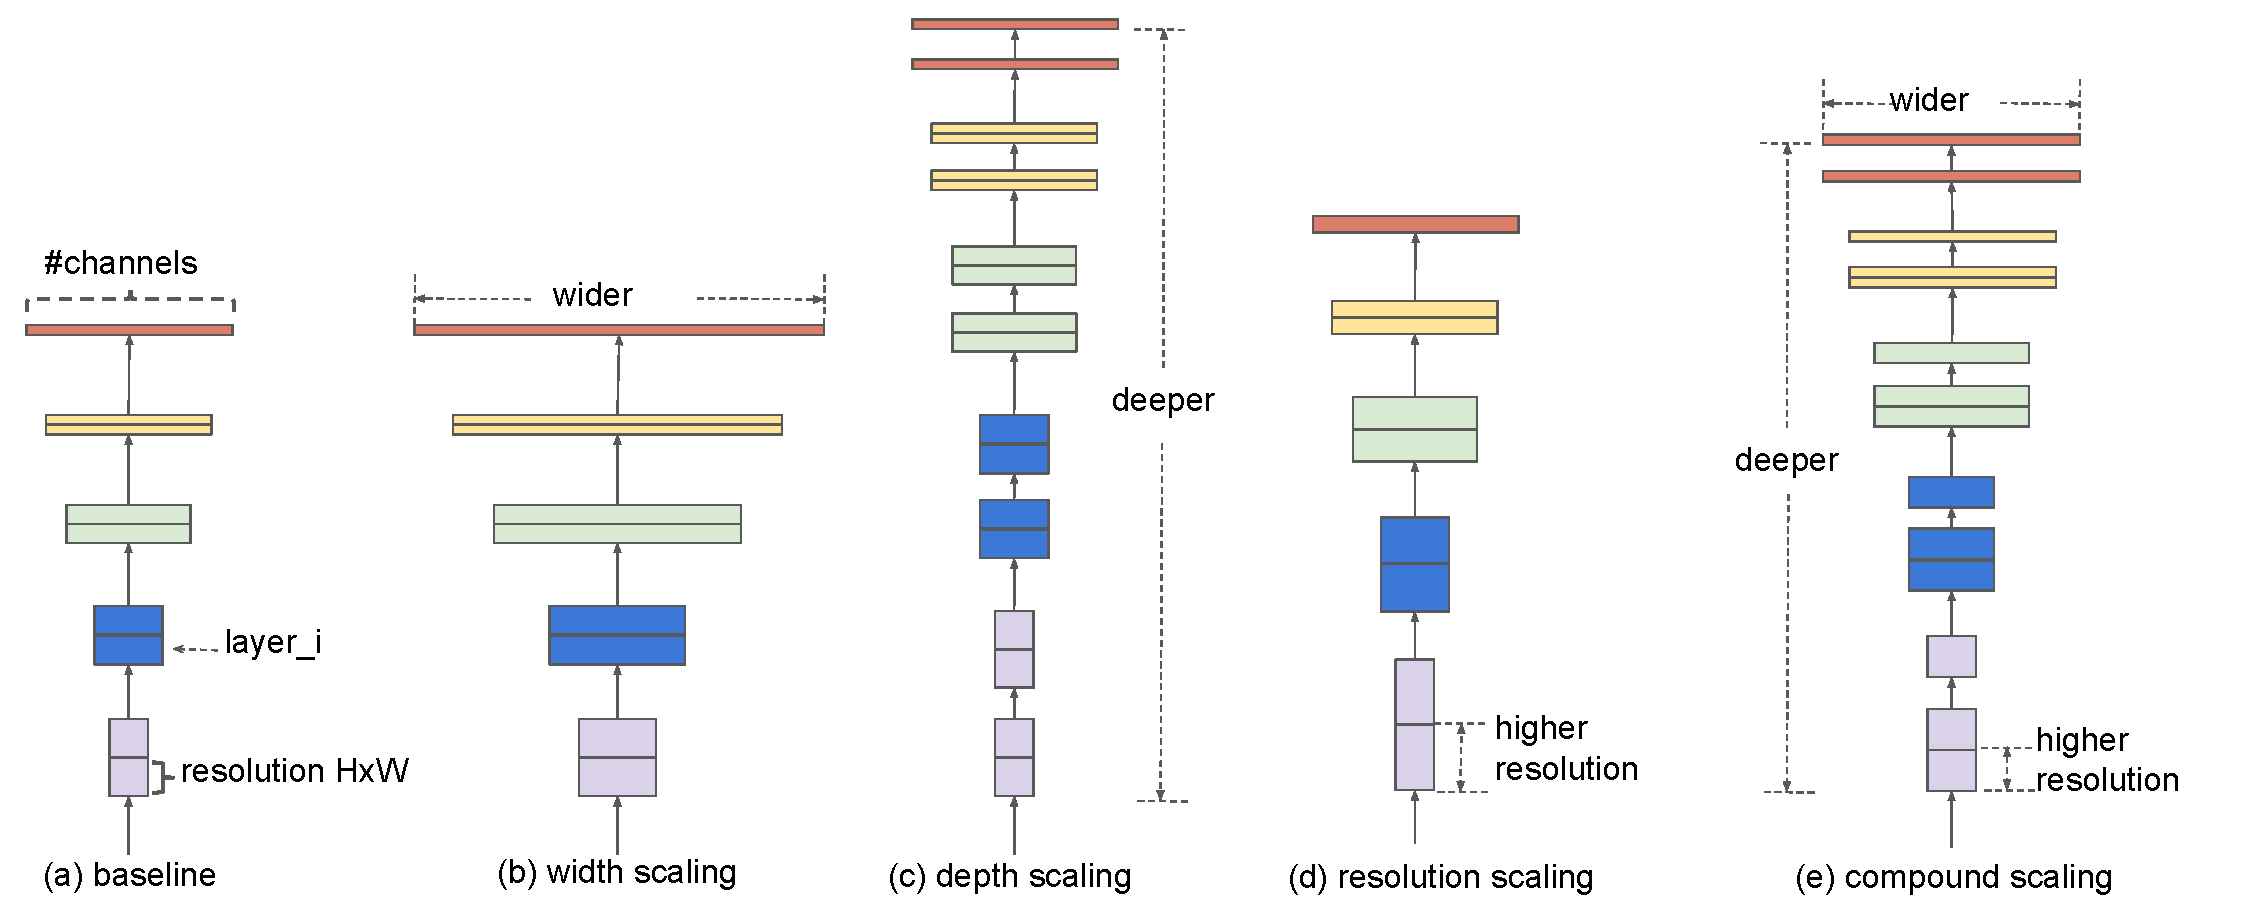
\includegraphics[width=0.81\textwidth]{figures/main/ch3-related_work/scalecompare.pdf}
  \caption{Illustration of the scaling of the EfficientNet architecture \cite{tan2019efficientnet}.}
  \label{figure:p1-ch3-illustration_efficientnet}
\end{figure}

Instead of compressing the model after the training step, researchers still tried to design architectures that are compact by nature but finding the best trade-off between depth, width and performance has proved to be a tedious work.
In order to scale the search, recent works have devised algorithms to automatically find the best architecture for a specific use case.
\citet{zoph2018learning,real2019regularized} have tried to tune the wide and depth of neural network architectures to obtain the best trade-off between efficiency and accuracy but these methods required a lot of manual tuning.
More recently, with a similar method, \citet{tan2019efficientnet} found a new compound scaling method to uniformly scales network width, depth, and resolution leading to groundbreaking result in terms of efficiency and accuracy (see Figure~\ref{figure:p1-ch3-illustration_efficientnet}).



% Therefore, do neural networks needs to be deep? \citet{ba2014deep} tried to answer this question and empirically demonstrated that shallow neural networks can learn the complex functions previously learned by another neural network. 
% This observation was then leveraged for compressing trained neural networks by~\citet{hinton2015distilling}.
% This technique called \emph{model distillation} consists to train a large complex model using all the available data and resources to be as accurate as possible, then a smaller and more compact model is trained to approximate the first model.
% While this approach for deployment purposes, it is needed to train one large network and one shallow  


% Scaling network width is commonly used for small size models \cite{mobilenetv117, mobilenetv218, mnas18}.
% As discussed in \cite{zagoruyko2016wide}, wider networks tend to be able to capture more fine-grained features and are easier to train. However, extremely wide but shallow networks tend to have difficulties in capturing higher level features.

% It is known that a network with a large enough single hidden layer of sigmoid units can \emph{theoretically} approximate any decision boundary~\cite{cybenko1989approximation}.

% It is known that a network with a large enough single hidden layer of sigmoid units can \emph{theoretically} approximate any decision boundary~\cite{cybenko1989approximation}.
% Therefore, do neural networks needs to be deep? 
% \citet{ba2014deep} tried to answer this question and empirically demonstrated that shallow neural networks can learn the complex functions previously learned by another neural network. 
% This observation was then leveraged for compressing trained neural networks by~\citet{hinton2015distilling}.
% This technique called \emph{model distillation} consists to train a large complex model using all the available data and resources to be as accurate as possible, then a smaller and more compact model is trained to approximate the first model.
% While this approach for deployment purposes, it is needed to train one large network and one shallow  


% First, a large complex model is trained using all the available data and resources to be as accurate as possible, then a smaller and more compact model is trained to approximate the first model.  
% The technique which was later specialized for deep learning models by~\citet{hinton2015distilling} (\aka model distillation) is often used to compress large ensemble models into compact single deep learning models.


% Do Deep Nets Really Need to be Deep?
% \cite{ba2014deep}
% In this paper we empirically demonstrate that shallow feed-forward nets can learn the complex functions previously learned by deep nets and achieve accuracies previously only achievable with deep models.

% Do Deep Convolutional Nets Really Need to be Deep (Or Even Convolutional)?
% \cite{urban2016deep}
%
% Deep, Skinny Neural Networks are not Universal Approximators?
% \cite{johnson2018deep}


% \cite{cybenko1989approximation}
% it was proved that a network with a large enough single hidden layer of sigmoid units can
% approximate any decision boundary 

% Instead of compressing the model after the training step, one can try to design models that are compact by nature (without compromising the generalization properties of the network).
% The benefit of this approach is that it reduces memory usage required during both training and inference.
% As a consequence, users can train models that are virtually larger using less time and less computing resources.
% They also save the trouble of training two models instead of one as it is done with distillation.

% Model Scaling: There are many ways to scale a ConvNet for different resource constraints: ResNet (He et al., 2016) can be scaled down (e.g., ResNet-18) or up (e.g., ResNet-200) by adjusting network depth (#layers), while WideResNet (Zagoruyko & Komodakis, 2016) and MobileNets (Howard et al., 2017) can be scaled by network width (#channels).
% It is also well-recognized that bigger input image size will help accuracy with the overhead of more FLOPS.
% Although prior studies (Raghu et al., 2017; Lin & Jegelka, 2018; Sharir & Shashua, 2018; Lu et al., 2018) have shown that network depth and width are both important for ConvNets’ expressive power, it still remains an open question of how to effectively scale a ConvNet to achieve better efficiency and accuracy. 

% pursue better accuracy and efficiency, it is critical to balance all dimensions of network width, depth, and resolution during ConvNet scaling.

% The number of parameters that is of interest for building compact neural network is the number of parameters needed to be saved in memory. 

% The number of parameters of a neural network is defined by the sum of the number of parameters of each layer which correspond to 
%
% The number of parameters of a neural network is dependent of three parameters: the dimension of the input (the resolution), the dimensions of the hidden layers and the depth of the network.
% More precisely, we can 
%
% The number of parameters of a neural network that is of interest is the number of parameters that we need to save in memory in order to perform the operations.

% Besides structured matrices, a variety of techniques have been proposed to build more compact deep learning models.
% These include \emph{model distillation}~\cite{hinton2015distilling}, tensor train~\cite{novikov2015tensorizing}, Low-rank decomposition~\cite{denil2013predicting}, to mention a few.
%
% However, circulant networks show good performances in several contexts (the interested reader can refer to the results reported by \citet{moczulski2016acdc} and \citet{thomas2018learning}).



%%%%%%%%%%%%%%%%%%%%%%%%%%%%%%%%%%%%%%%%%%%%%%%%%%%%%%%%%%%%%%%%%%%%%%%%%%%%%%%%
\section{Position of the Contribution Regarding the State-of-the-Art}
\label{section:p1-ch3_position_of_the_contributions_regarding_the_state-of-the-art}
%%%%%%%%%%%%%%%%%%%%%%%%%%%%%%%%%%%%%%%%%%%%%%%%%%%%%%%%%%%%%%%%%%%%%%%%%%%%%%%%


In the previous sections, we show the current methods and techniques for designing compact and efficient neural networks. 
Mainly, three techniques exist.
The first one considers the use of specific memory representation as well as efficient data structures.
This technique is interesting and has the advantage to be applicable to any neural networks, therefore is complementary to other methods.
The second method consists of using structured linear layers to reduce the number of parameters and leverage fast matrix-product algorithms. 
Finally, recent works devised efficient and compact neural network architectures by tuning the width and depth parameters of neural networks.
It is now clear that convolutional neural networks are state-of-the-art for image classification and detection.
Moreover, recent architectures~\cite{tan2019efficientnet} have been found with architecture search algorithms and have very competitive results. 
However, neural networks based on structured matrices (different than convolution) can still be interesting for other use cases or small-footprint deep learning like smartphone or IoT devices. 

Our contributions on \emph{Deep Diagonal Circulant Neural Networks} are a direct follow-up to the work of~\citet{cheng2015exploration,sindhwani2015structured,moczulski2016acdc,thomas2018learning} focusing on compact neural networks with \emph{structured matrices}.
Although, this diagonal circulant layers fit in the low displacement rank framework, we demonstrate much better performances in practice.
Indeed, thanks to a solid theoretical analysis and thorough experiments, we were able to train deep (up to 40 layers) circulant neural networks (see Chapter~\ref{chapter:diagonal_circulant_neural_network}), and apply, for the first time, this structured architecture in the context of large-scale video classification (see Chapter~\ref{chapter:diagonal_circulant_neural_networks_for_video_classification}).
Note that we are able to train \emph{fully structured networks} (\ie, networks with structured layers only) hence demonstrating that diagonal circulant layers are able to model complex relations between inputs and outputs.
This contrasts with previous experiments in which only one or a few dense layers were replaced inside a large redundant network such as VGG~\cite{simonyan2014very}.
To the best of our knowledge, this is the first time such networks can be trained.  




